%% This is an example first chapter.  You should put chapter/appendix that you
%% write into a separate file, and add a line \include{yourfilename} to
%% main.tex, where `yourfilename.tex' is the name of the chapter/appendix file.
%% You can process specific files by typing their names in at the 
%% \files=
%% prompt when you run the file main.tex through LaTeX.
\chapter{VM2Docker}
\label{chap:vm2docker}
In this chapter, we outline the design and implementation of the VM2Docker system. In section~\ref{sec:usecases}, we discuss typical use cases for VM2Docker. In section~\ref{sec:sysoverview} we outline and diagram the system as a whole. The system itself consists of two major components: filesystem conversion, as discussed in section~\ref{sec:fsconversion}, and process detection, as described in section~\ref{sec:pdetection}. Finally, we conclude with a brief discussion of the system's technical specifications in section~\ref{sec:techspecs}.

\section{Use Cases}
\label{sec:usecases}
Overall VM2Docker has a number of theoretical and practical use cases where it might be particularly effective. We target single and multi-purpose virtual machines that run standard, unprivileged processes. Notably, the primary prerequisite is that any process or application running in the VM must also be able to function correctly in a headless Linux container. This excludes GUI applications, although they could theoretically be supported through a tool such as Docker Desktop \cite{ddesktop}. This also excludes any VMs that use custom modifications to the kernel or have privileged access to special devices on the host. As of Docker 1.2, custom privileges can also be added to containers to parallel those specified for a given VM on a case by case basis, but this generally breaks the complete isolation that Docker provides between containers.

Examples of such virtual machines that would be capable of being converted to a container are the following:
\begin{itemize}
\item Web server
\item Database
\item Mail server
\item Git server
\item Hadoop node
\item Cluster or grid computing node
\item Other non-UI computing
\end{itemize}

In all of these cases, VM2Docker will succeed in converting a given set of hosts to their corresponding, automatically layered Docker images. The goal of the layering is to maximize the size and quantity of layers that are shared in common among the different virtual machines. Since Docker retains just one copy of each layer on disk, regardless of how many images use the layer, the total disk space used by the converted containers will be less than that used by the original VMs. Furthermore, when run, the containers will achieve performance benefits of running on the lightweight Docker framework as compared to their original, fully-isolated and less performant VM environments. A full analysis and evaluation of the improved disk usage of VMs converted with VM2Docker is provided in chapter~\ref{chap:eval}.

%\section{Usage \& Configuration}
%%%%%%%%%%
\section{System Overview}
\label{sec:sysoverview}
In this section, we outline the design and implementation of the VM2Docker framework. The filesystem conversion process is broken down into three important steps. First, as outlined in section~\ref{sec:osdetection}, we determine the OS and distribution running on each VM and matches it up with a given Docker base image. Second, as described in section~\ref{sec:packagemanagement}, we assemble one or more additional layers corresponding to the packages that are installed in each VM. Finally, we apply a diff-based algorithm to create a layer that contains all other files that haven't yet been accounted for but were on the original VM filesystem. The next component of the VM conversion process consists of container configuration. VM2Docker automatically determines which processes are running on each host, along with the commands to run them, and maps them to commands to be run in a corresponding Dockerfile. Exposed ports are automatically detected and opened on the given containers, and container resources are allocated based on the resources present in the initial VM.

\begin{figure}[h]
\centering
    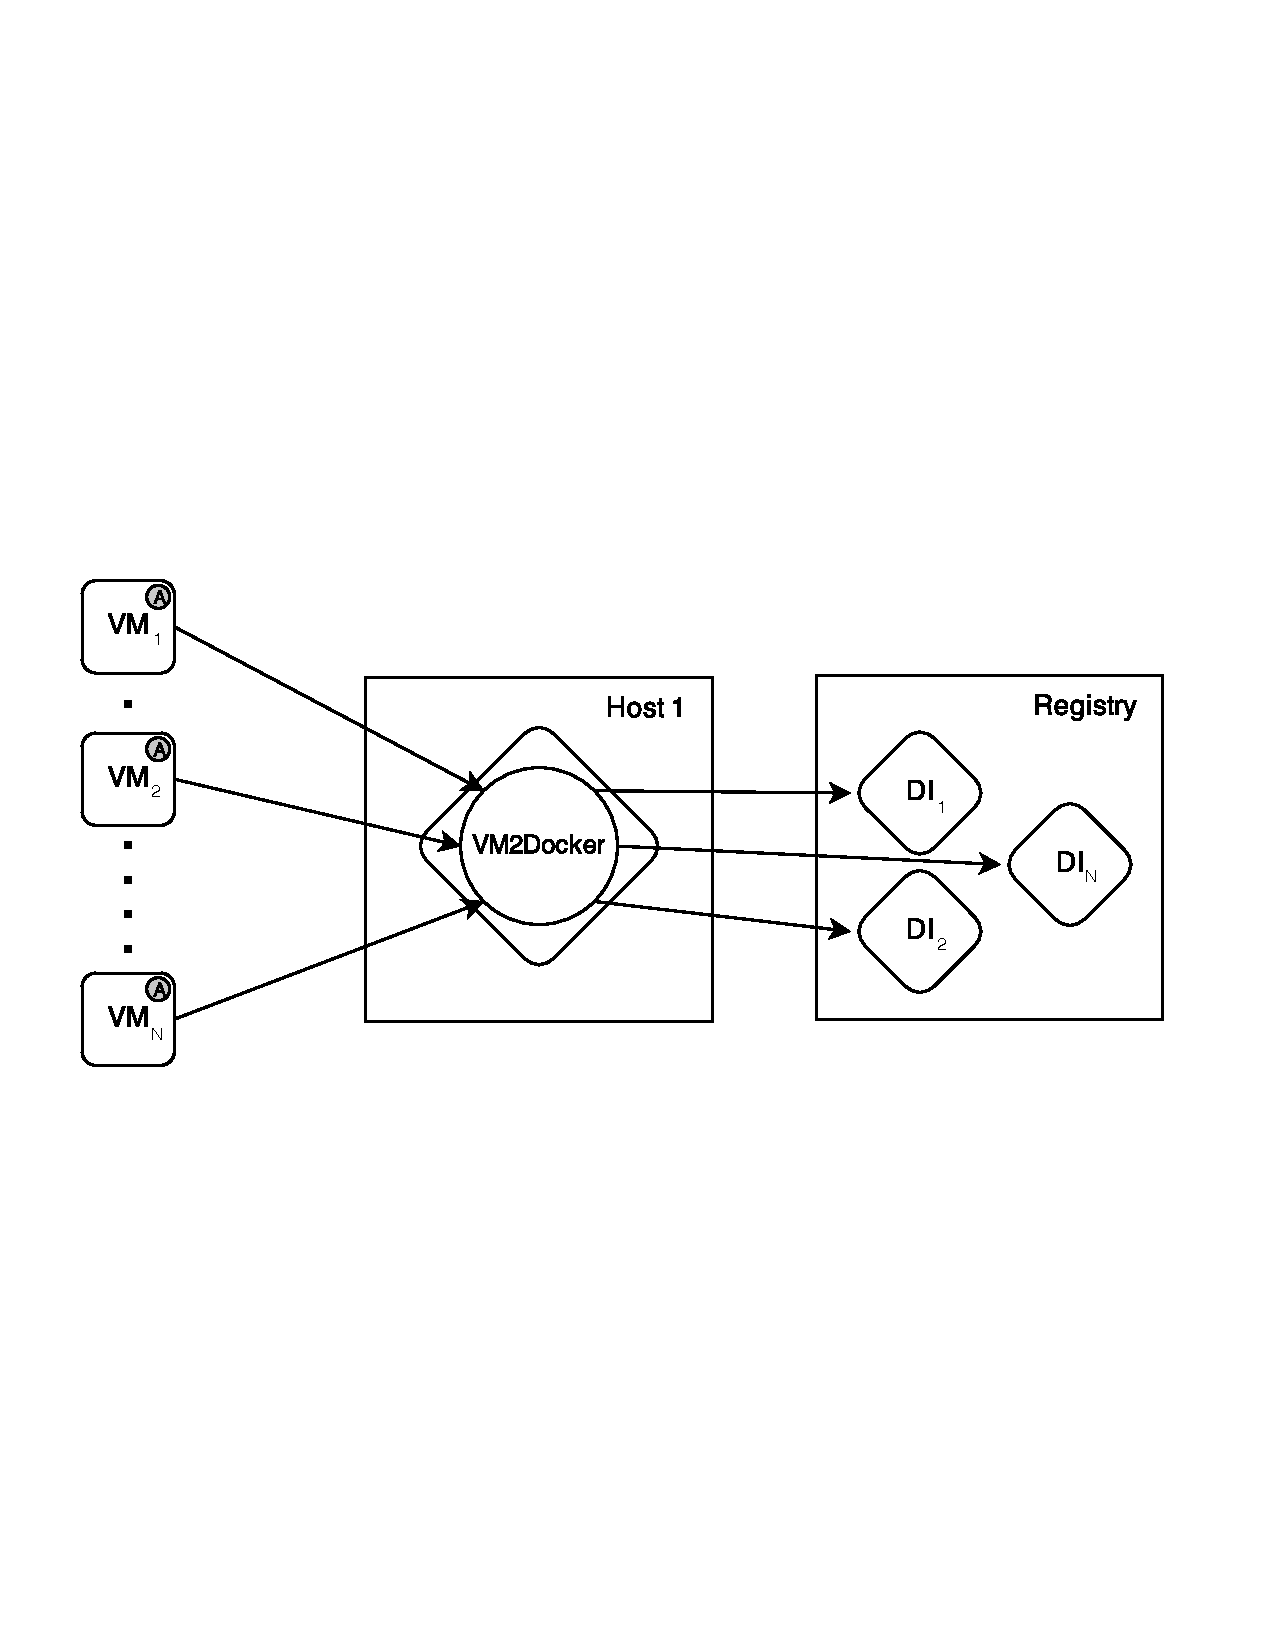
\includegraphics[width=1.0\textwidth]{system2.pdf}
    \caption{The following diagram illustrates an overview of the system and how the VM2Docker framework interacts with the virtual machines provided as input and converts them to corresponding Docker images. The rounded squares represent the input virtual machines and the rounded diamonds represent the resulting Docker images. To be converted, each VM must be running an instance of the "agent", as described in section~\ref{sec:agent}, and identified by a gray circle with the letter "A." The "chief," which initiates the conversion and is identified by the circle labeled VM2Docker, is itself a Docker image and can therefore be run on any host that has Docker installed. The resulting Docker images are deployed to a Docker registry, which can either be hosted on Host 1 or a separate host entirely. }
   \label{fig:sys}
\end{figure}
\subsection{Chief + Agent}
\label{sec:agent}
As displayed in figure~\ref{fig:sys}, the VM2Docker framework is divided into two components: the chief and the agent. The chief is centrally deployed on a single server which initiates the conversion. The agent is a self-contained executable that is deployed and run on each VM that needs to be converted. The chief communicates with the agent on each VM in order to convert them to their corresponding, layered, Docker images.  

\section{Filesystem Conversion}
\label{sec:fsconversion}
A significant component of this endeavor comprises the optimal decomposition of a virtual machine into a set of configuration files and an associated Dockerfile, which together can be used to build a Docker image. Docker`s filesystem layering allows multiple images that inherit from the same parent image to share many of the same files, therefore drastically cutting down on the total space needed for many copies or minor derivations of the same base image. In addition to space savings, the corresponding Docker images take up a fraction of the space of a VM and can therefore be downloaded and shared in a much more convenient manner.

Starting from the original VM, VM2Docker will apply a set of transformations in order to decompose the VM's filesystem into a set of layers, which, together, make up the original filesystem. At the end of the automatic layering process, a filesystem diff is created and applied from the topmost Docker layer to the original VM filesystem. This ensures that after the diff is applied, the Docker image is byte for byte equivalent to the original VM's filesystem. Figure~\ref{fig:layering} depicts how three such virtual machines, all running the same operating system and release, might share certain layers in common after being converted to the Docker format.

\begin{figure}[h]

\centering
    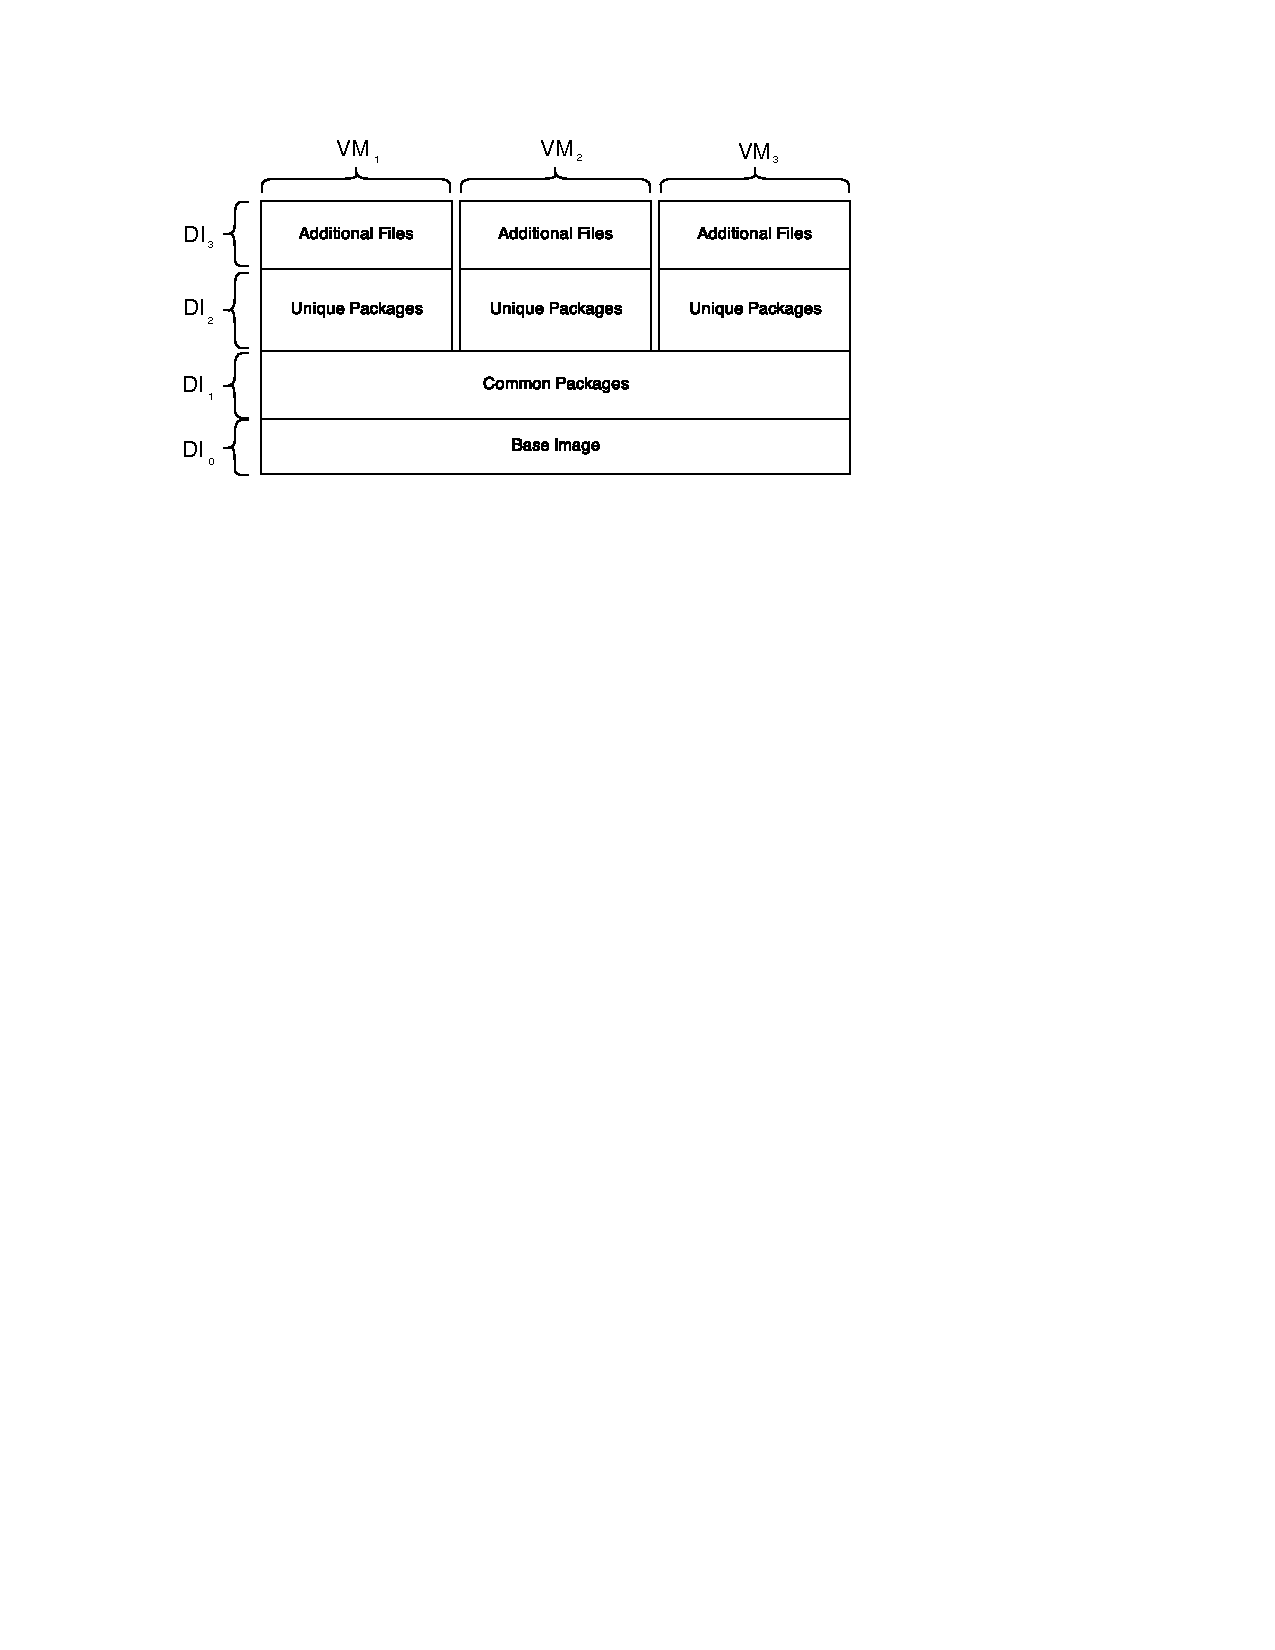
\includegraphics[width=0.7\textwidth]{layering.pdf}
    \caption{An example of how VMDocker layers the filesystems of three virtual machines running the same operating system and release. Docker will keep only one copy of layers $DI_0$ and $DI_1$, because each of the three VMs share these in common.}
\label{fig:layering}
\end{figure}

\subsection{Base Image}
\label{sec:osdetection}
The most straightforward way of exploiting layering in Docker is by means of simple Docker image inheritance. Built into the engine is a method by which each image can be told to start from an existing image, identified by a repository and tag name. This could either be a base image corresponding to a specific release of an operating system, or it could be a more complex image, which itself inherits from another image.

We make use of this layering by automatically detecting the distribution and release of the corresponding VM. As long as the VM is running a release of Linux with a kernel version that exceeds 3.8, it should be supported by VM2Docker. The distribution and release can be found in \texttt{/etc/*-release} and roughly correspond to the repository and tag name, respectively. Once obtained, we check for the existence of the corresponding base image on the Docker Registry. For now, we are using the publicly available registry but intend to transition to a private registry. A private registry would allow any such base images that are not available on the public registry, like RedHat because of licensing reasons, to be generated on the fly with a tool like \texttt{debootstrap} \cite{debootstrap} and then pushed to the registry for future availability.

\subsection{Package Management}
\label{sec:packagemanagement}

To increase the number of layers and maximize the sharing of these layers across different Docker images, we make aggressive use of package detection and installation. Each OS has a slightly different package management tool, so VM2Docker abstracts out the particular commands for a given tool and is therefore extensible regardless of the operating system in use. We have tested and implemented code that works for Ubuntu, Mageia, and CentOS, which use \texttt{apt-get}, \texttt{urpmi}, and \texttt{yum}, respectively.

We maximize layers in common by first computing the intersection of packages for all VMs of the same operating system and release. This set of packages is culled using dependency detection, which is described below. Once filtered, a Dockerfile is constructed that inherits from a given base image and contains instructions to install all packages in common.

This process is repeated a second time for each VM using the remaining packages that have not yet been installed. A Dockerfile is generated that inherits from the image created in the previous step and installs the remaining packages specific to this VM. Note that if there is only one VM of a given operating system and release, these two layers will be the same.

Presumably, the package installation process will consist only of package installs, but it is conceivably possible that there are some installed on the base image, but not the VM, which would lead to a Dockerfile instruction to uninstall the given packages.

The goal of this technique is to coerce the Docker image filesystem to be as similar to the original VM as possible before calculating the diff, thereby reducing its size.

\subsubsection{Dependency Detection}
\label{sec:depdetection}
A useful feature of VM2Docker that greatly reduces the number of packages installed and increases Dockerfile readability is its ability to reduce the number of packages listed to be installed within a given Dockerfile without affecting correctness.

Many packages installed on a given OS are never directly installed. Instead, they are installed as a result of satisfying a dependency for another package. In other words, even if explicit instructions to install these packages are not given, the end result is the same. VM2Docker takes advantage of this observation and the resulting improvements are incredibly effective, as shown in the evaluation section in table~\ref{table:culling}.

To accomplish this dependency-safe reduction in packages, we generate a directed graph of all the packages that will be installed, where there is an edge from $A$ to $B$ if and only if package $A$ depends on package $B$. Once generated, the only packages that need to be directly installed are those that have an in-degree of 0 or are a part of a strongly connected component of size greater than 1. The addition of the strongly connected component requirement takes into account the possibility of dependency cycles, in which packages will have an in-degree of greater than 0 but still must be included in the install list. See figure~\ref{fig:depgraph} for a visual representation of such a directed graph.

\begin{figure}[h]
\centering

    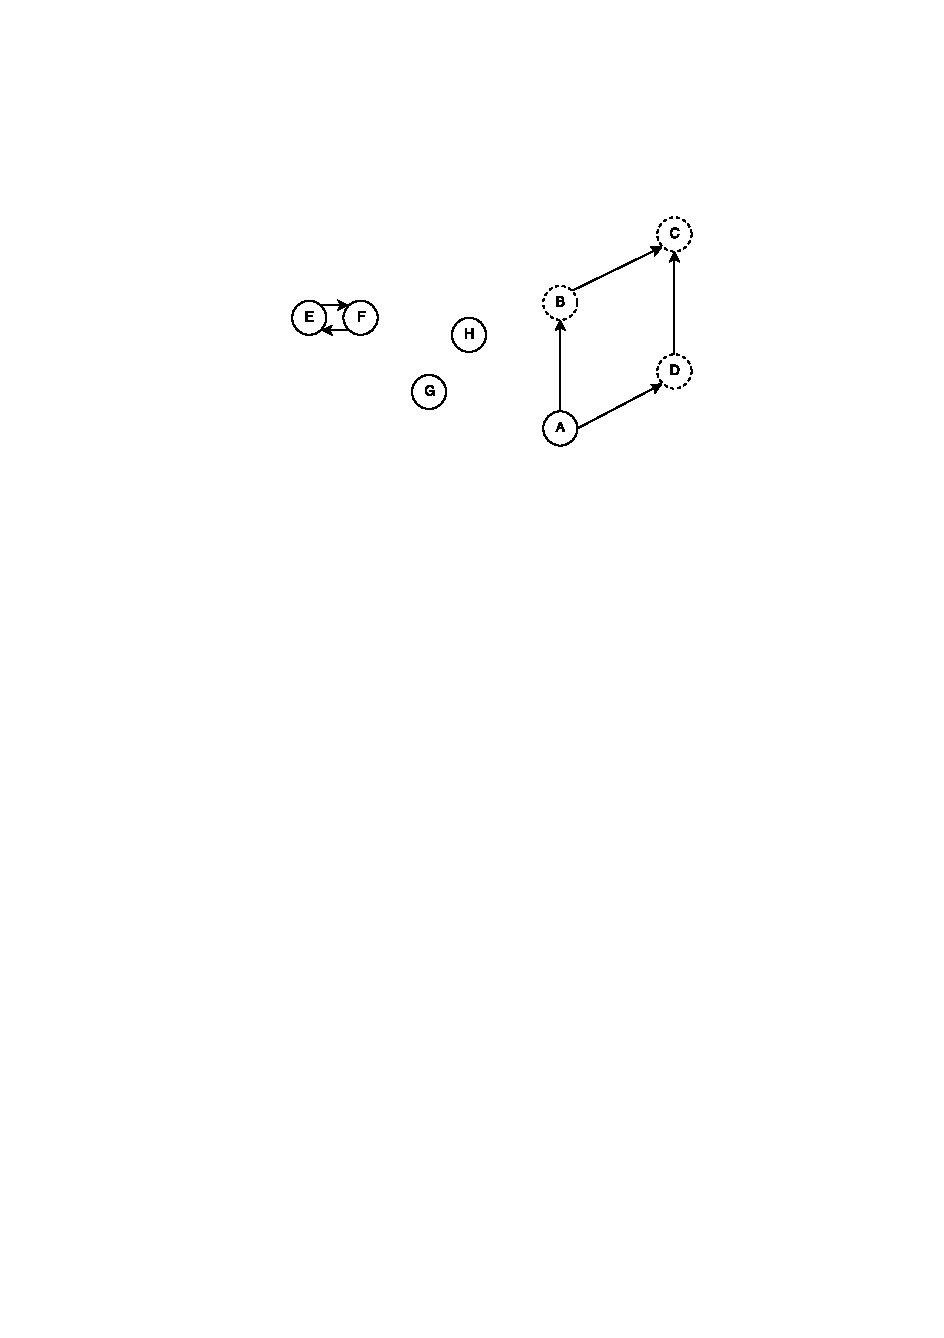
\includegraphics[width=.6\textwidth]{depgraph.pdf}
    \caption{In the example above, packages $A$-$G$ are pictured. Package $X$ depends on package $Y$ if and only if there is a directed edge from $X$ to $Y$. Of those pictured, packages $B$, $C$, and $D$ do not need to be installed because during installation of package $A$, the package manager will detect that $B$ and $D$ are uninstalled dependencies, and that $C$ is recursively a dependency of them. Packages $E$ and $F$ still need to be included, even though their in-degree is bigger than 0, because they are a strongly connected component on which no other installed nodes depend. All those packages that are removed from the list of packages to be installed are pictured with a dashed line circle, while the packages that can't be removed are pictured with a solid line circle.}
   \label{fig:depgraph}
\end{figure}

\subsection{Diff}
\label{sec:diff}
The topmost layer of the Docker image consists of all the files needed such that the entire filesystem is byte-by-byte equivalent to the original VM filesystem. This is accomplished by calculating a filesystem diff from the existing Docker image, with all packages installed, to the original VM filesystem. The Dockerfile is given instructions to inherit from the Docker image completed in the previous step, equipped with all packages installed, and then to apply the diff to the filesystem, thereby recovering the complete VM filesystem. There are a number of different strategies for computing this diff, each with its own benefits and drawbacks. We analyzed two in particular: \texttt{rsync} and \texttt{rdiffdir}, and VM2Docker is fully extensible to support other algorithms with very little user intervention and a simple subclass.


\underline{rsync}\\
\texttt{rsync} is a backup tool used to sync changes to and from a remote server. It can also be used between directories on the same host. Two rounds of rsync are needed in order to account for additions and modifications, as well as deletions. The first round, from Docker image to the VM filesystem, represents all of the changes and additions that need to be added to the Docker image to get to the VM. The second round, which we run in reverse, gives us the set of changes and deletions that have been applied. Cross-referencing these lists, we extract just the deletions and convert them to a list of the filepaths of the deleted files. We create a tarball of all of the changes and additions. To build the final Docker image, we expand the tarball and then iterate through the list and delete each file listed. This yields the filesystem of the original VM. 

\texttt{rsync} has the benefit of being a native C executable that is bundled with almost  every Linux system. The one major drawback is how it handles file modifications. Since the diff is represented as a set of files in directories, it has no way of indicating which components of a file have changed without copying the modified file in its entirety. This can be especially wasteful if a large file has only a few bytes modified. While the \texttt{rsync} algorithm is optimal about remote backups in only sending the changed version of a file and patching it on the other side, running \texttt{rsync} for two directories on the same host does not have the same sort of optimizations.

\underline{rdiffdir}\\
\label{sec:rdiffdir}
\texttt{rdiffdir} is a tool based on \texttt{rdiff} but that can be used for directories as well. The \texttt{rdiff} tool is an independent implementation of the \texttt{rsync} algorithm that generates delta files that can then be used to patch the existing file without the target file present. For example, if \texttt{rdiff} generates a delta file from $A$ to $B$. \texttt{rdiff} can use the delta to patch $A$ and recover file $B$, even if $B$ is no longer present. The \texttt{rdiff} algorithm uses a fixed size window to generate rolling hashes of a given file in order to generate these deltas in an optimal manner.

Use of \texttt{rdiffdir} generally allows for more optimal, smaller diffs to be created, thereby resulting in more portable Docker build instructions. The one major drawback of using \texttt{rdiffdir} is its non-native implementation. As a component of the Duplicity framework, \texttt{rdiffdir} is written in Python and therefore has some pre-existing dependencies. While the generating of the Delta file happens within the VM2Docker chief environment where dependencies are less important, the patching of the filesystem using the generated delta occurs in the resulting Docker container environment. If a given VM did not already have it installed, \texttt{rdiffdir} would need to be installed, the patch applied, and then uninstalled, which is a lot less straightforward than the expansion of a tarball as seen in the \texttt{rsync} example.


\subsection{Dockerfiles}
The instructions to build a given Docker image are provided in a corresponding Dockerfile. Starting from the base image, which we will call $DI_0$, VM2Docker generates a Dockerfile with a set of instructions that denote how to generate the next layer, given the current one. Figure~\ref{fig:dockerfiles} depicts this progression of Docker images, and how the Dockerfiles ($DF$) bridge the gap between them.

\begin{figure}[h]

\centering
    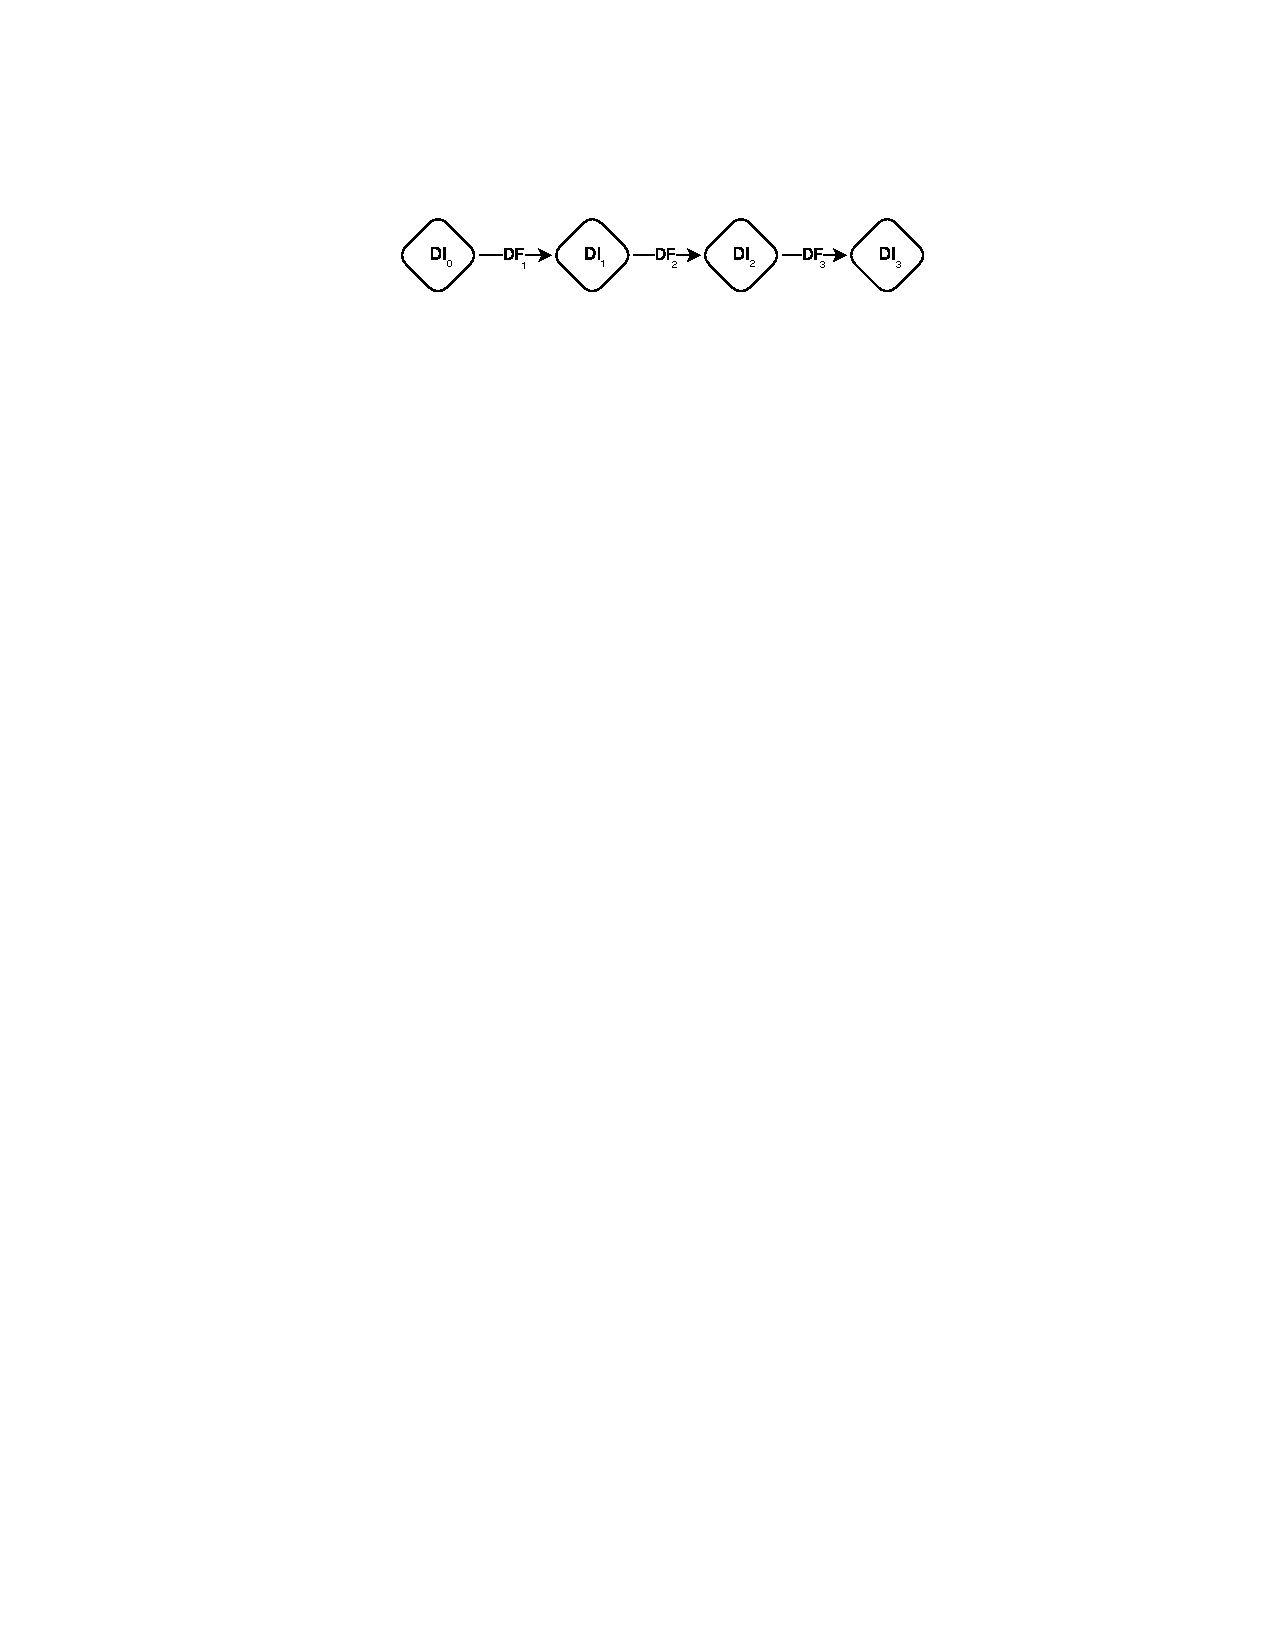
\includegraphics[width=0.7\textwidth]{dockerfiles.pdf}
    \caption{An example of the Docker image build process and the set of instructions used to get between images. Starting from the base image, $DI_0$, Docker generates image $DI_1$ by executing instructions contained in $DF_1$.}
\label{fig:dockerfiles}
\end{figure}

Depending on the operating system and the diff algorithm specified, VM2Docker generates the appropriate commands and inserts them into the Dockerfiles, along with the auxiliary delta file in the case of $DF_3$. When built, the Docker images are generated and take the inheritance scheme as pictured in figure~\ref{fig:dockerfiles}.


\subsection{Verification}

With all of these filesystem transformations in place, it is essential to verify that the Docker image that is built is identical to the original VM in terms of its filesystem. Since the diff operation is always executed last, the resulting patch should always restore the final filesystem to be a byte-for-byte identical copy as the original VM filesystem. Even if the process of installation or uninstalling packages selects the wrong ones, the worst that can happen is an increase in the size of the diff layer, which does not affect the correctness of the system.

For completeness, we implement an optional flag that can be enable a verification tool to be run with the virtual machine conversion. After conversion is complete, it will build the final Docker images and export them to disk. The resulting Docker images are identical to the VM if and only if the filesystem diff between the Docker image filesystem and the original VM filesystem is the empty set.

\subsection{Additional Space-Reducing Techniques}
\label{sec:addnltechs}
Certain files in the VM are either unnecessary, or can be regenerated on the fly. Since Docker containers share their kernel with the host operating system, they disregard any kernel modules that are provided in the container. Thus, we can safely remove these associated files from the diff in order to save space. Furthermore, the package repository cache takes up a fair amount of space, and is used only for performance reasons. This can be safely purged from the filesystem without affecting correctness. For Ubuntu, these files are located at \texttt{/var/cache/apt/pkgcache.bin} and \texttt{/var/cache/apt/srcpkgcache.bin} and can potentially take up about 100 MB.

\section{Process Detection}
\label{sec:pdetection}
In addition to converting the filesystem to one that may better exploit layering, another big component of VM2Docker is its ability to automatically configure the resulting containers in a manner similar to that of the original VM.

Unlike VMs which start up an entire operating system, Docker containers are started by running a specific command in the shell. VM2Docker maps each running process on a host to a new container. In this paradigm, the command that runs the container corresponds to the command to start up the given process, and each VM may potentially map to multiple containers. Although technically feasible, VM2Docker may not always work with multi-process VMs, depending on the level and type of interprocess communication occurring between the isolated processes. Further research into multi-container orchestration is discussed in section~\ref{sec:future}.

The VM2Docker agent, which runs directly on the host with root privileges, can automatically detect the currently running processes that were kickstarted at startup, as well as the commands used to start them using \texttt{ps}. Furthermore, we use \texttt{netstat} to determine which processes are bound to which ports, to be sure to expose the corresponding ports through Docker. The agent also reads information available in the \texttt{proc} pseudo-filesystem in order to determine the current working directory and environment variables of the given process. All of this information is transmitted to the chief over a socket and is used during the container configuration component of the conversion process.

Finally, in terms of resource allocation, the VM2Docker agent reads from the \texttt{/proc} pseudo file-system and parses the information available in \texttt{meminfo} and \texttt{cpuinfo}. This information is passed over a socket to the VM2Docker chief during conversion in order to provide the container with the same resource restrictions and allocations as its corresponding VM.

\section{Technical Implementation \& Specifications}
\label{sec:techspecs}
The VM2Docker chief is written as a Python script and is made to communicate with one or more VM2Docker agents. Each agent is a simple executable, written in C, and is compiled to the appropriate architecture and OS, depending on the VM. The C agent sets up a TCP socket through which the chief can communicate via a custom remote procedure call protocol. This protocol is responsible for transmitting the entire filesystem, checking app dependencies, and getting specific runtime information about the process that will be running within the container. In order to be platform independent, the VM2Docker chief is bundled with an associated Dockerfile such that the conversion process happens within Docker container. This allows for all dependencies to be automatically and seamlessly installed. The entire conversion process is therefore platform agnostic and requires only the Docker environment as well as a target Docker host and/or registry to store the newly created Docker images and optionally run them. Thus, VM2Docker makes use of Docker's ability to run inside of itself \cite{dockerindocker}. Prior to making this design decision, an early prototype of VM2Docker instead took as argument the filepath to the root of the VM's filesystem. This required a separate VM to be running the same operating system as the VM to be converted, which proved unwieldy for each additional operating system attempted. Furthermore, since we had only access to the filesystem, process detection was not possible either. The current chief and agent design overcomes both of these challenges. 

An additional technical challenge was determining the protocol to be used to respond to remote procedure calls to the agent over the socket. These calls returned both plain text, as well as raw data in the case of the filesystem transmission, of arbitrary length back to the chief for processing. To handle the incoming data, we designed a reusable ring buffer in Python with a seamless interface that provided methods for reading until a specified single or multi-byte delimiter. The protocol we chose makes use of the null byte as a delimiter for text. In the case of a file, a header is sent that specifies the number of bytes to read after the header, while ignoring any occurrences of the delimiter. This abstraction allowed us to effectively and seamlessly handle the transmission of data from agent to chief.

\subsection{Usage}

%TODO: technical challenges


The prototype of VM2Docker is available at \url{https://github.com/ecbtln/vm2docker}.
